\chapter{Results}

\section{Extracting Object Sizes}

In \fullref{sec:determining_obj_size}, we proposed three methods for determining object size by extracting data from the \emph{Scene Graph} \citep{xu2017scenegraph} dataset. In this section, we compare and evaluate the three methods.

\subsection{Evaluation}

The size data extracted from the \emph{Scene Graph} \citep{xu2017scenegraph} dataset using the above method are compared against the hand-written sizes. The extracted absolute sizes can be directly compared to the hand-written data. The relative sizes are compared against size ratios between the absolute hand-written sizes.

\medskip

We use the Root-Mean-Square Error (RMSE) as a metric. For $N$ predictions $y_0, \dots, y_n$ and target values $t_0, \dots, t_n$, RMSE is defined as:
\begin{align*}
    \text{RMSE} = \sqrt{\frac{1}{n}\sum_{i = 0}^n (y_i - t_i)^2}
\end{align*}

\medskip

The second metric we are interested in is the percentage of covered pairs, i.e., for how many pairs, out of the total of $119\,025$ pairs, we were able to extract the size data.

\subsection{Quantitative and Qualitative Results}

The RMSEs of the proposed size extraction methods are reported in Tables \ref{tab:sizeextraction:1} and \ref{tab:sizeextraction:2}. \Cref{tab:sizeextraction:1} compares variants of the proposed methods with transitive closures.

\begin{table}[!ht]
    \centering
    \resizebox{\textwidth}{!}{
        \begin{tabular}{c|c|c|c}
            \textbf{Method} & \textbf{Width RMSE} & \textbf{Height RMSE} & \textbf{Pairs Covered} \\
            \hline \hline
            Absolute                            & $51.93$           & $43.17$           & $\textbf{91.49\%}$    \\ 
            Relative                            & $\textbf{12.97}$  & $16.46$           & $7.50\%$              \\
            Relative + word embedding           & $43.93$           & $42.46$           & $63.60\%$             \\
            Relative + word embedding (0.85)    & $19.78$           & $24.87$           & $10.34\%$             \\
            Relative + word embedding (0.95)    & $13.13$           & $\textbf{16.12}$  & $7.92\%$              \\
        \end{tabular}
    }
    \caption[Comparison of the size extraction methods]{Comparison of the size extraction methods.}
    \label{tab:sizeextraction:1}
\end{table}

\begin{table}[!ht]
    \centering
    \resizebox{\textwidth}{!}{
        \begin{threeparttable}
            \begin{tabular}{c|c|c|c}
                \textbf{Method} & \textbf{Width RMSE} & \textbf{Height RMSE} & \textbf{Pairs Covered} \\
                \hline \hline
                Absolute$^*$                        & $51.93$           & $43.17$           & $91.49\%$         \\ 
                Relative                            & $\textbf{43.65}$  & $\textbf{41.04}$  & $79.70\%$         \\
                Relative + word embedding           & $55.53$           & $47.92$           & $\textbf{100\%}$  \\
                Relative + word embedding (0.85)    & $53.35$           & $45.65$           & $86.57\%$         \\
                Relative + word embedding (0.95)    & $49.39$           & $42.03$           & $82.30\%$         \\
            \end{tabular}
            \begin{tablenotes}
            \small
            \item $^*$ Transitive closure cannot be applied to the absolute sizes. The results are the same as in \Cref{tab:sizeextraction:2}. For the sake of comparison, they are also included in this table.
            \end{tablenotes}
        \end{threeparttable}
    }
    \caption[Comparison of the size extraction methods with transitive closure]{Comparison of the size extraction methods with transitive closure.}
    \label{tab:sizeextraction:2}
\end{table}

All relative size methods outperformed the absolute size method in terms of RMSE. However, these methods cover significantly fewer pairs. The transitive closure partially solves the small pair coverage problem, but it also introduces larger errors. Similarly, the word embeddings helped to increase both the pair coverage and errors.

\begin{figure}[ht]
    \centering
        \begin{subfigure}{0.45\textwidth}
            \centering
            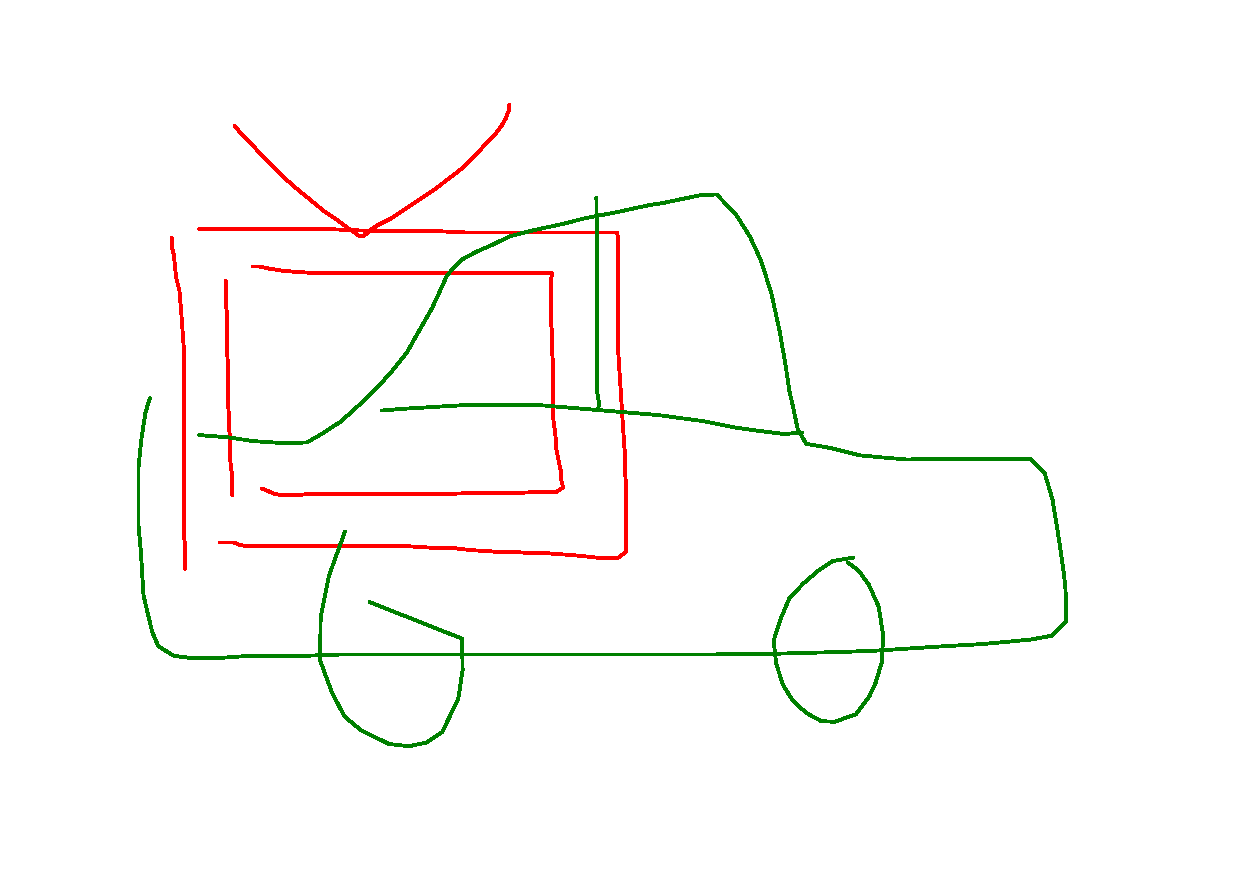
\includegraphics[width=\textwidth]{figures/car_on_tv_abs.pdf}
        \end{subfigure}
        \begin{subfigure}{0.45\textwidth}
            \centering
            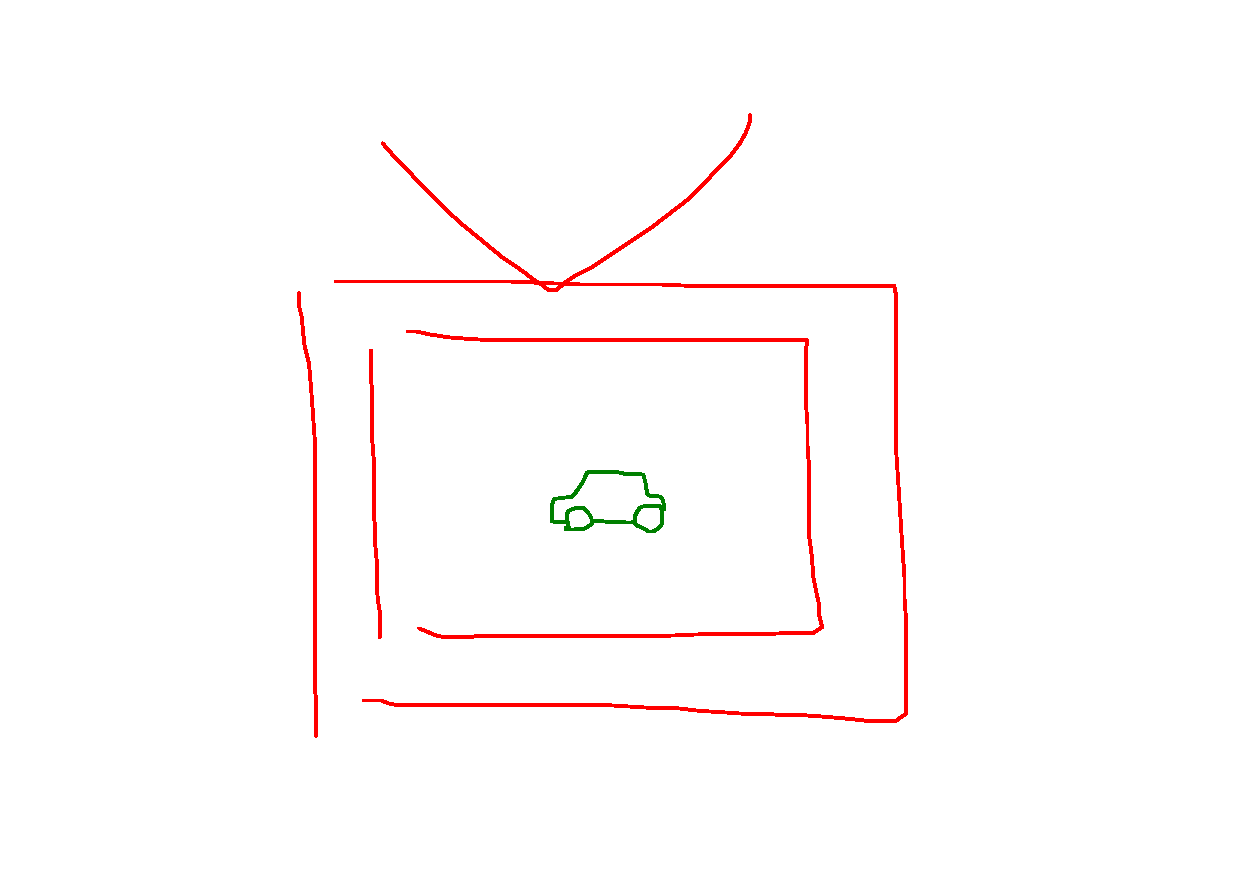
\includegraphics[width=\textwidth]{figures/car_on_tv_rel.pdf}
        \end{subfigure}
    \caption[Comparison of absolute and relative size method]{Drawings generated from description \protect\say{A car is on the television.} using absolute (right) and relative (left) sizes.}
    \label{fig:absolute_vs_relative}
\end{figure}

\begin{figure}[ht]
    \centering
    \captionsetup[subfigure]{labelformat=empty}
        \begin{subfigure}{0.45\textwidth}
            \centering
            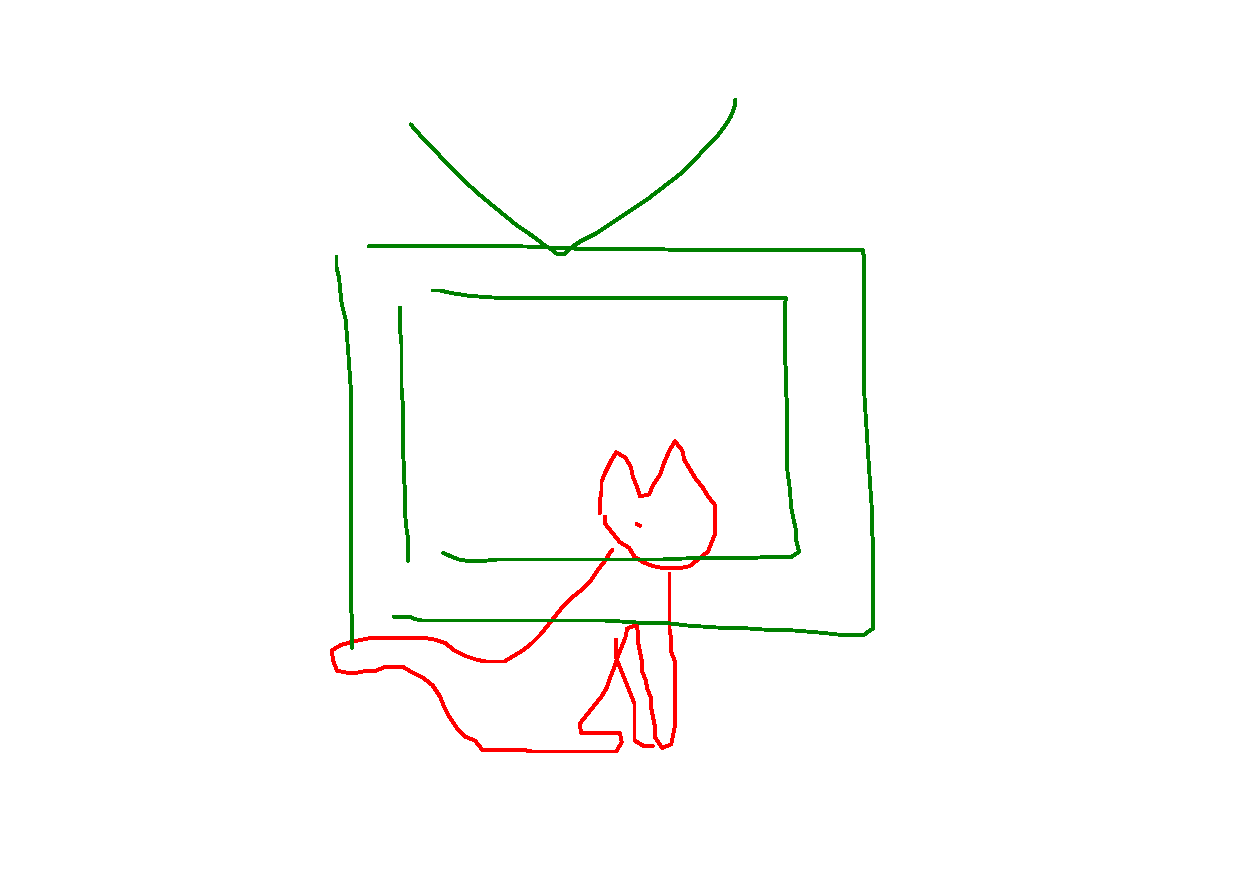
\includegraphics[width=\textwidth]{figures/television_behind_cat.pdf}
            \caption{\protect\say{A television is behind a cat.}}
        \end{subfigure}
        \hfill
        \begin{subfigure}{0.45\textwidth}
            \centering
            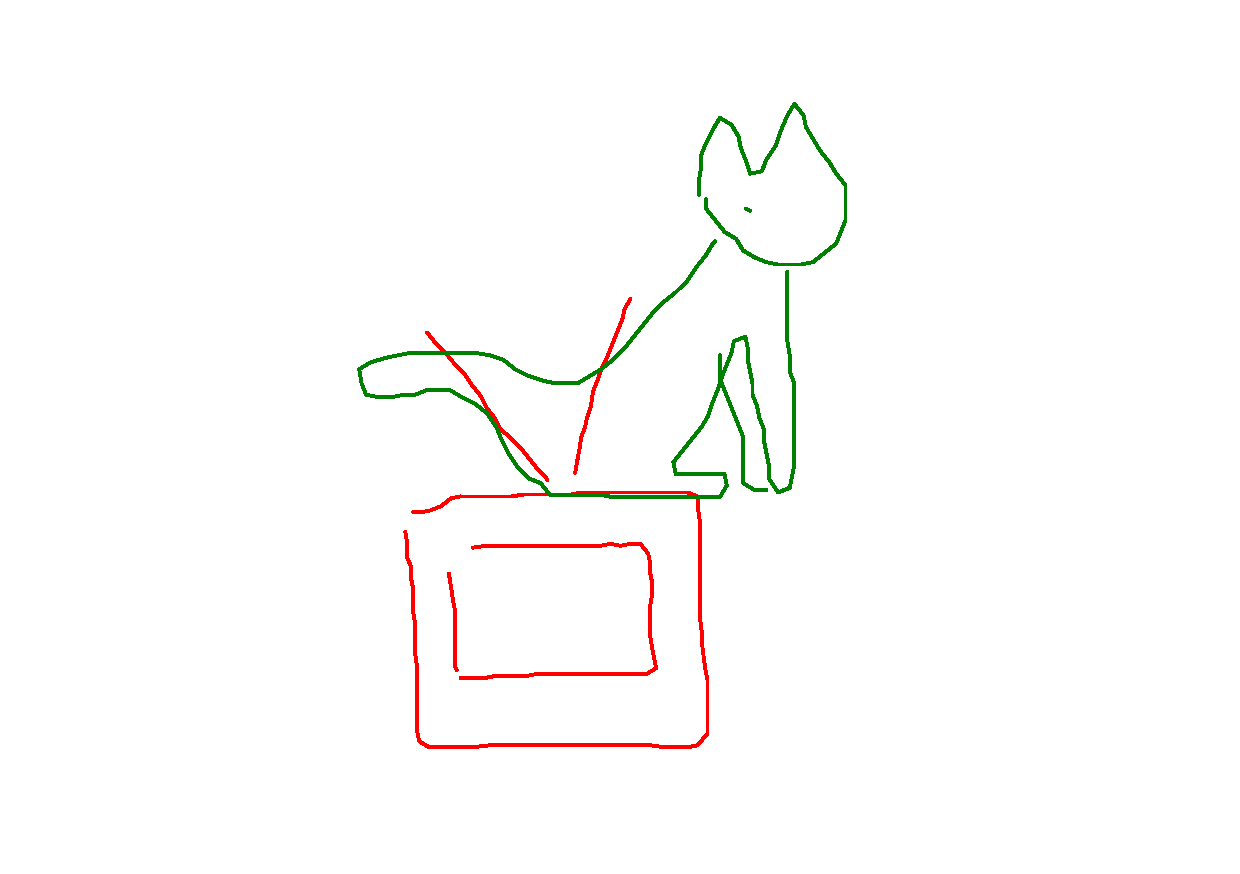
\includegraphics[width=\textwidth]{figures/cat_on_television.pdf}
            \caption{\protect\say{A cat is sitting on a television.}}
        \end{subfigure}
        
        \begin{subfigure}{0.45\textwidth}
            \centering
            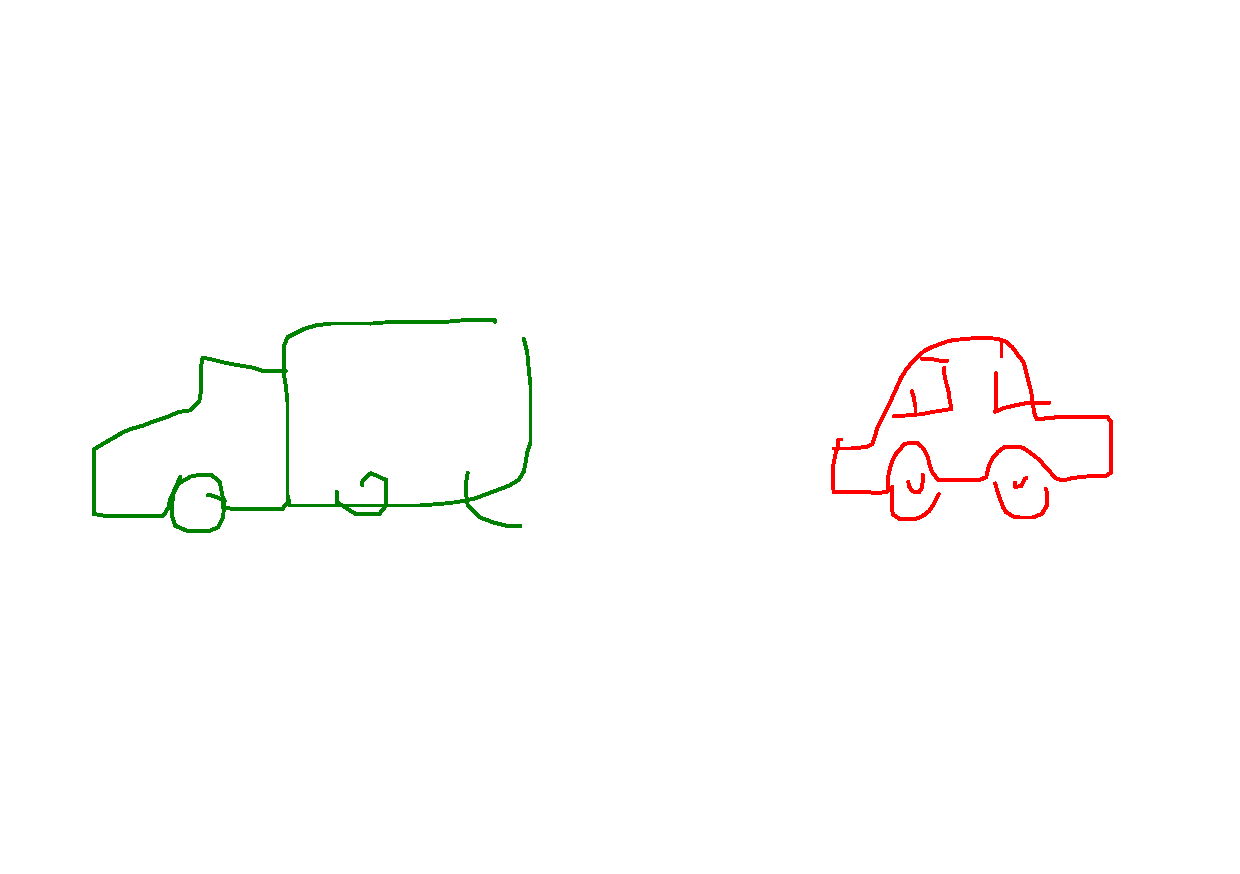
\includegraphics[width=\textwidth]{figures/truck_behind_car.pdf}
            \caption{\protect\say{A truck is behind a car.}}
        \end{subfigure}
        \hfill
        \begin{subfigure}{0.45\textwidth}
            \centering
            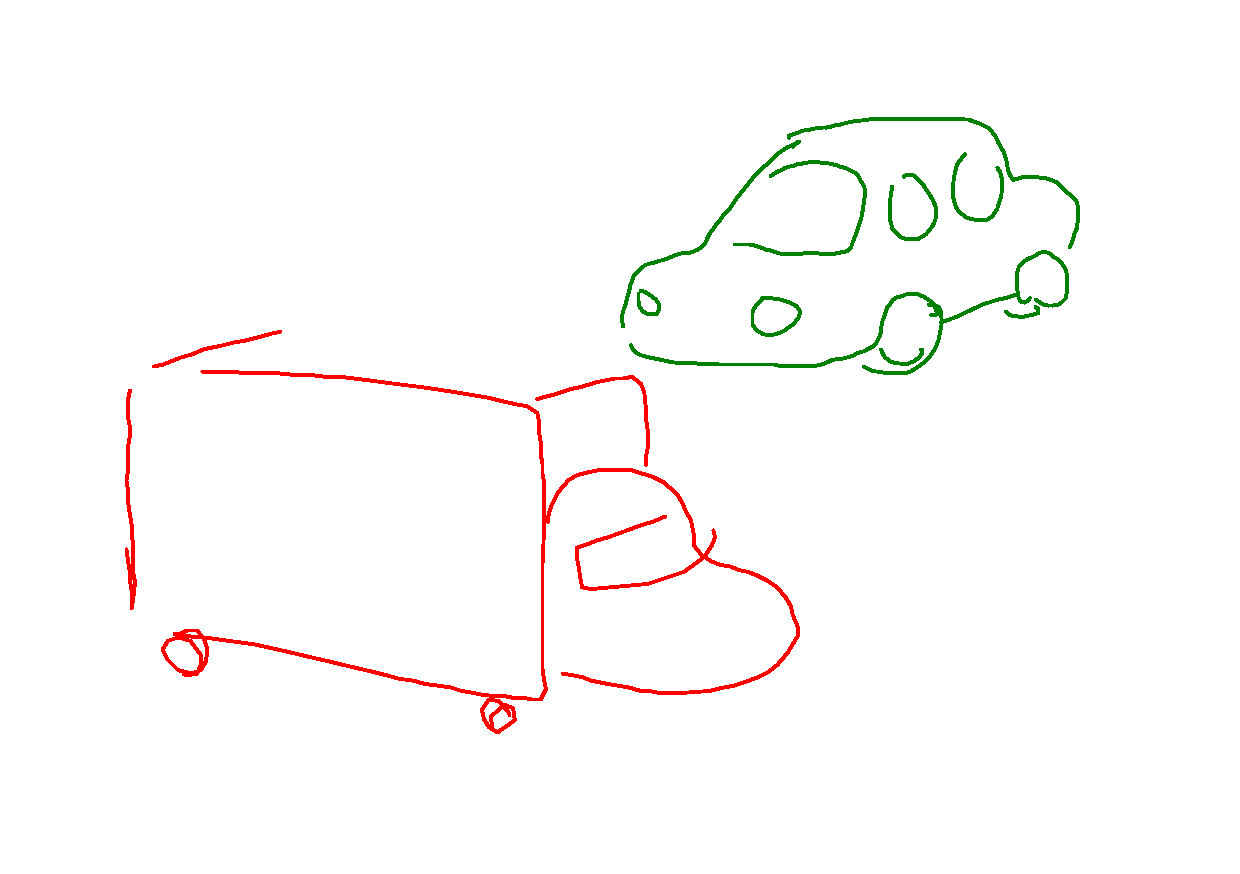
\includegraphics[width=\textwidth]{figures/car_next_to_truck.pdf}
            \caption{\protect\say{A car is next to a truck.}}
        \end{subfigure}
       
        \begin{subfigure}{0.45\textwidth}
            \centering
            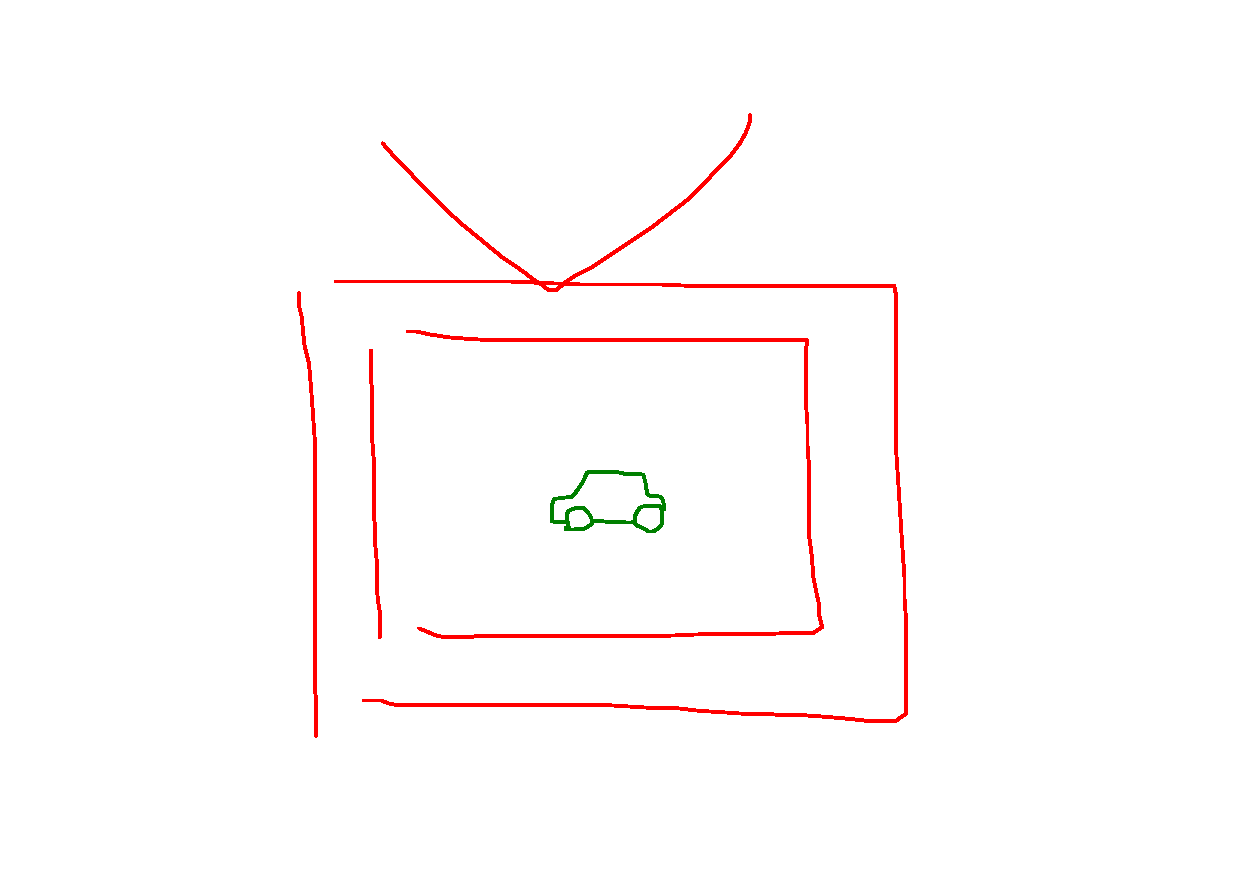
\includegraphics[width=\textwidth]{figures/car_on_tv_rel.pdf}
            \caption{\protect\say{A car is on the television.}}
        \end{subfigure}
        \hfill
        \begin{subfigure}{0.45\textwidth}
            \centering
            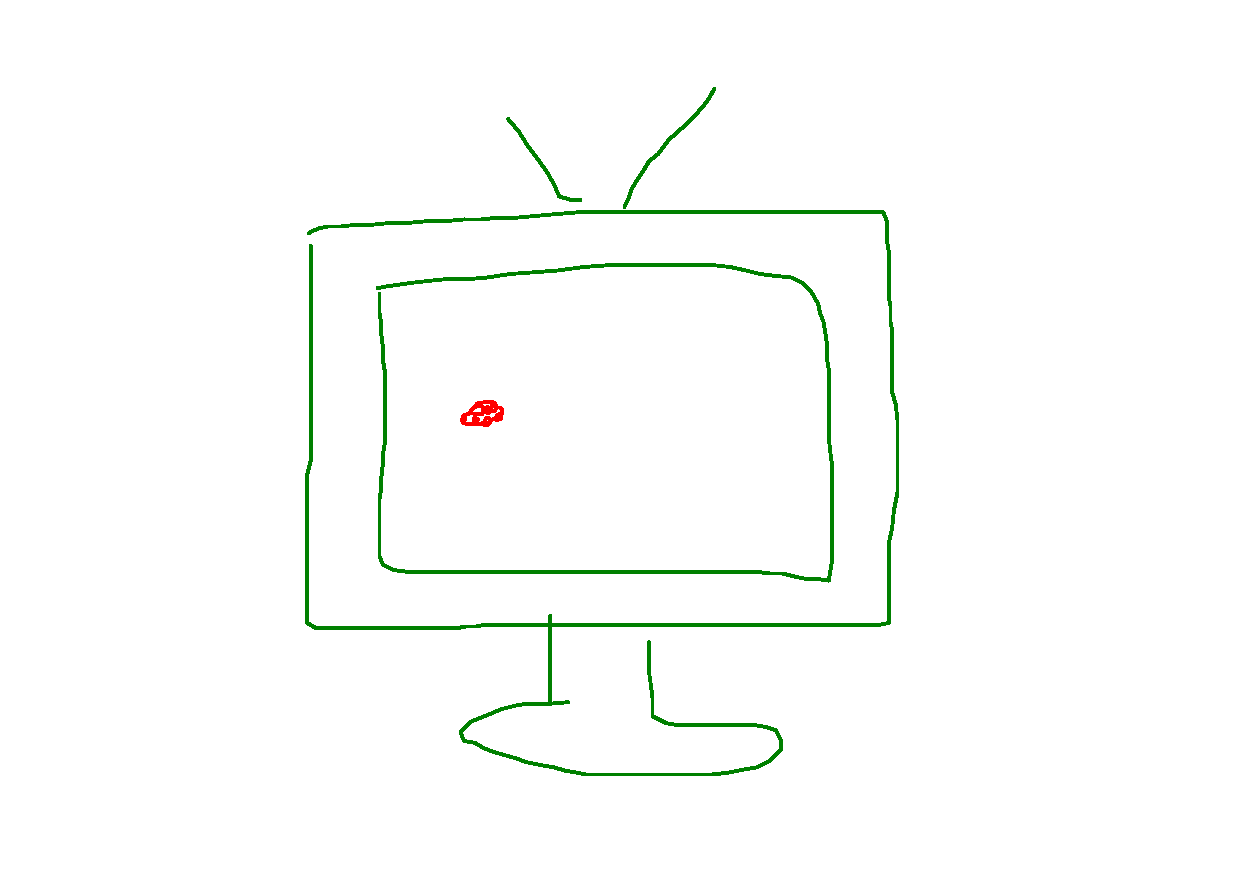
\includegraphics[width=\textwidth]{figures/television_in_front_of_car.pdf}
            \caption{\protect\say{A television is in front of a car.}}
        \end{subfigure}
    \caption[Drawings generated using the relative size method]{Drawings generated using the relative size method.}
    \label{fig:relative_size_examples}
\end{figure}

\Cref{fig:absolute_vs_relative} compares the absolute size and relative size methods on the example given in \Cref{sec:determining_obj_size}. In this particular example, the relative size method addresses the problem stated in the mentioned section. However, the rightmost drawing in \Cref{fig:relative_size_examples} shows that the method fails the other way around. Presumably, the dataset captures certain pairs of objects only in a narrow variety of contexts, leading to biased estimations. Furthermore, the relative size approach is oblivious to the predicates associated with the relation. We have chosen not to include the predicate as it would vastly decrease the pair coverage.

\section{Positional Constraints}
\label{sec:constraint_results}

In \Cref{sec:rule_based_constraints} and \Cref{sec:classifier_based_constraints}, we introduced a rule-based and a classifier-based approach for determining the objects' positions. In this section, we compare those two approaches.

\medskip

The first version of the classifier-based approach considers only the predicate and the relative position described in \Cref{sec:classifier_based_constraints}. As shown in \Cref{fig:boundaries:3}, constraints implemented using this classifier closely resemble the rule-based alternatives. It shows that the \emph{Scene Graph} \citep{xu2017scenegraph} dataset is a viable source of semantic information about the connection of predicates and mutual positions of objects. The figure also suggests that this classifier is a sufficient replacement for the simple rule-based approach.

\medskip

The second version of the classifier takes into account the semantic subject. \Cref{fig:boundaries:2} shows that this classifier can capture different semantics of a predicate with respect to the subject. More examples are shown in \Cref{fig:boundaries:5}. 

\medskip

The major drawback of the classifier-based approach is the lack of information about the shape of the object. This problem is partially illustrated by \Cref{fig:boundaries:4}. In some cases, the rule-based approach provides more precise boundaries than the classifier-based alternative.

\begin{figure}[ht]
    \centering
        \begin{subfigure}{0.45\textwidth}
            \centering
            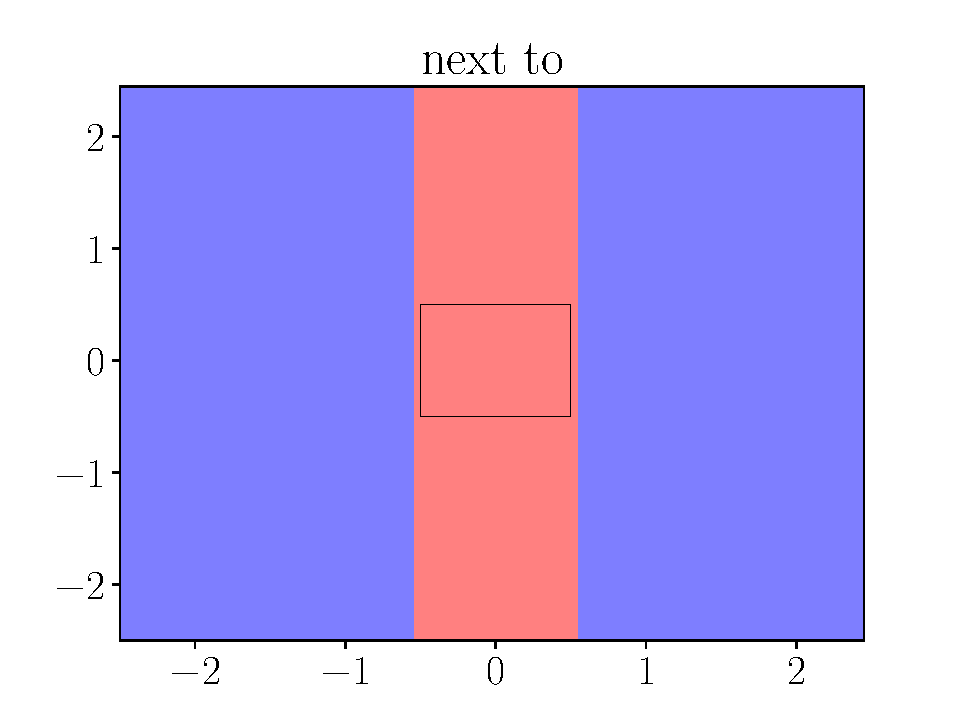
\includegraphics[width=\textwidth]{figures/next_to_rule.pdf}
        \end{subfigure}
        \begin{subfigure}{0.45\textwidth}
            \centering
            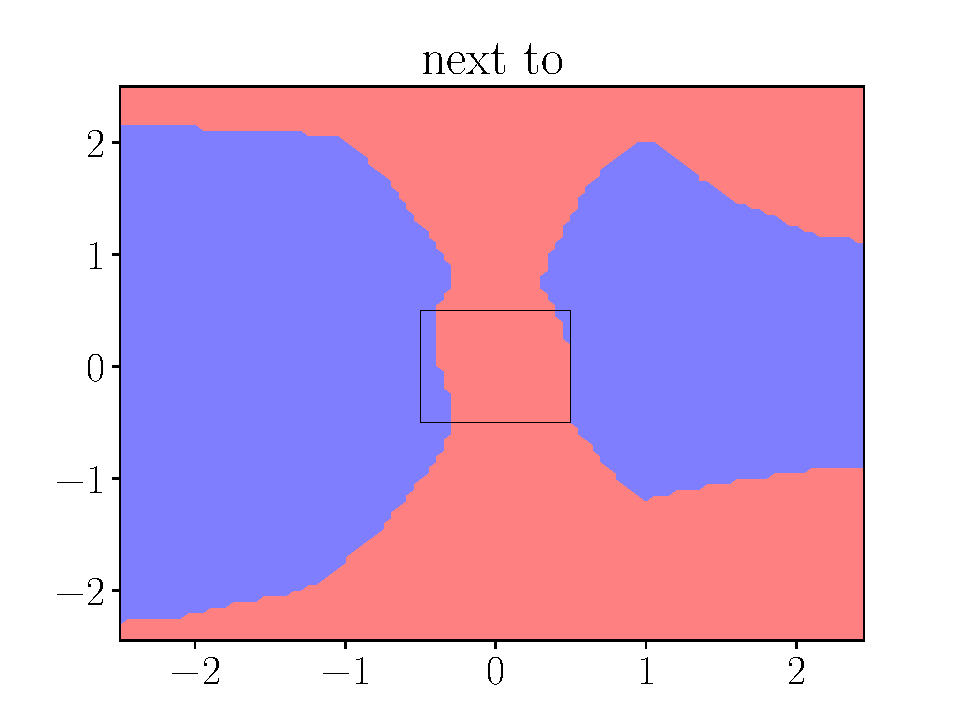
\includegraphics[width=\textwidth]{figures/next_to_predicate_only.pdf}
        \end{subfigure}
        \begin{subfigure}{0.45\textwidth}
            \centering
            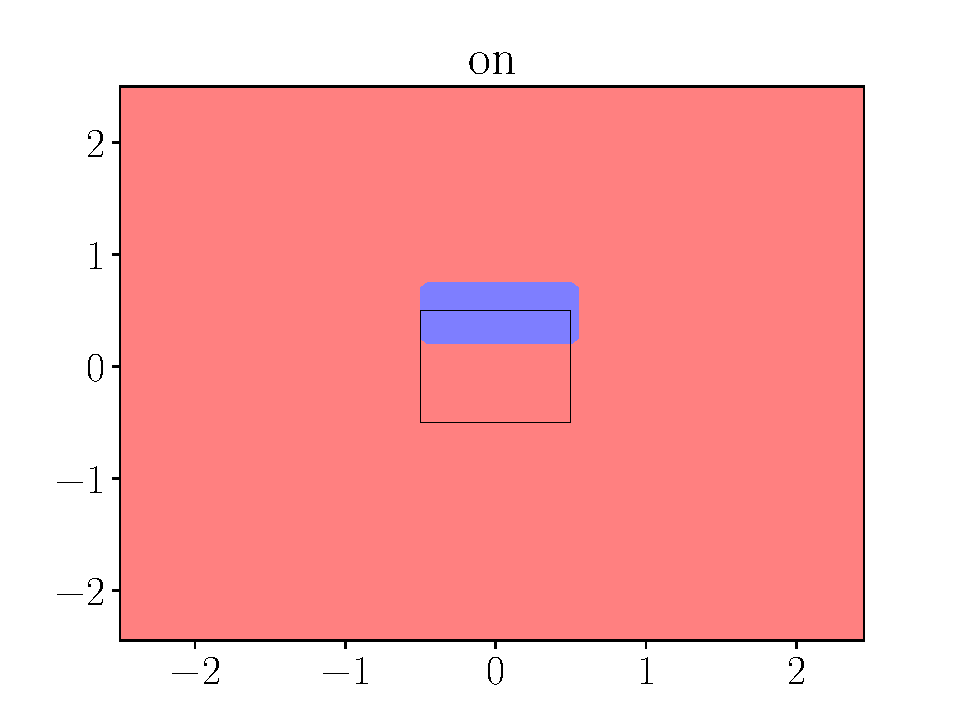
\includegraphics[width=\textwidth]{figures/on_rule.pdf}
        \end{subfigure}
        \begin{subfigure}{0.45\textwidth}
            \centering
            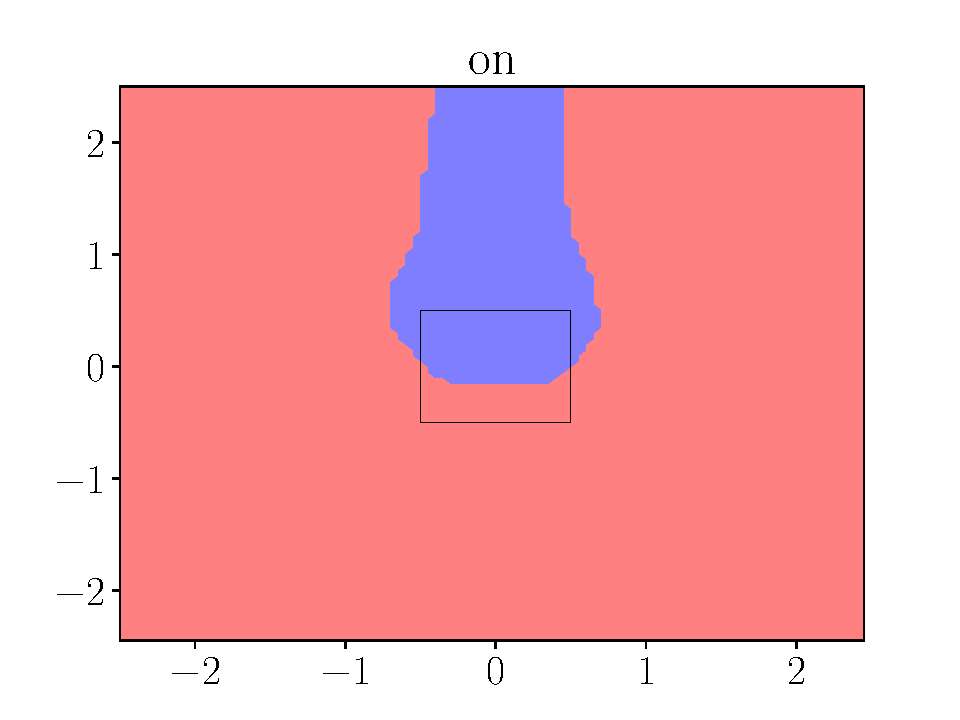
\includegraphics[width=\textwidth]{figures/on_predicate_only.pdf}
        \end{subfigure}
        \begin{subfigure}{0.45\textwidth}
            \centering
            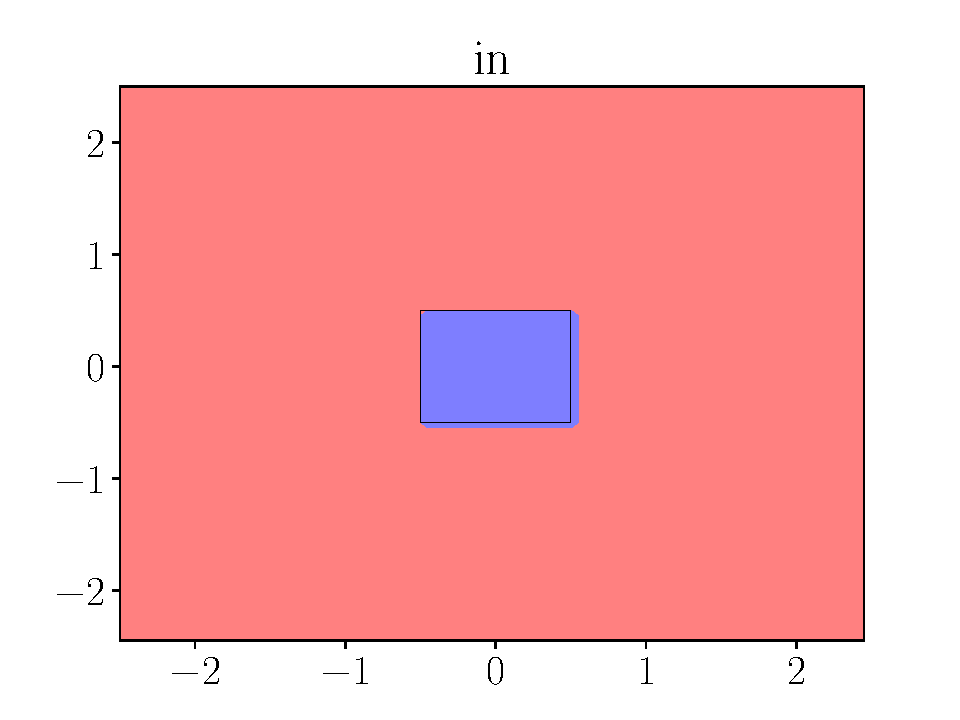
\includegraphics[width=\textwidth]{figures/in_rule.pdf}
        \end{subfigure}
        \begin{subfigure}{0.45\textwidth}
            \centering
            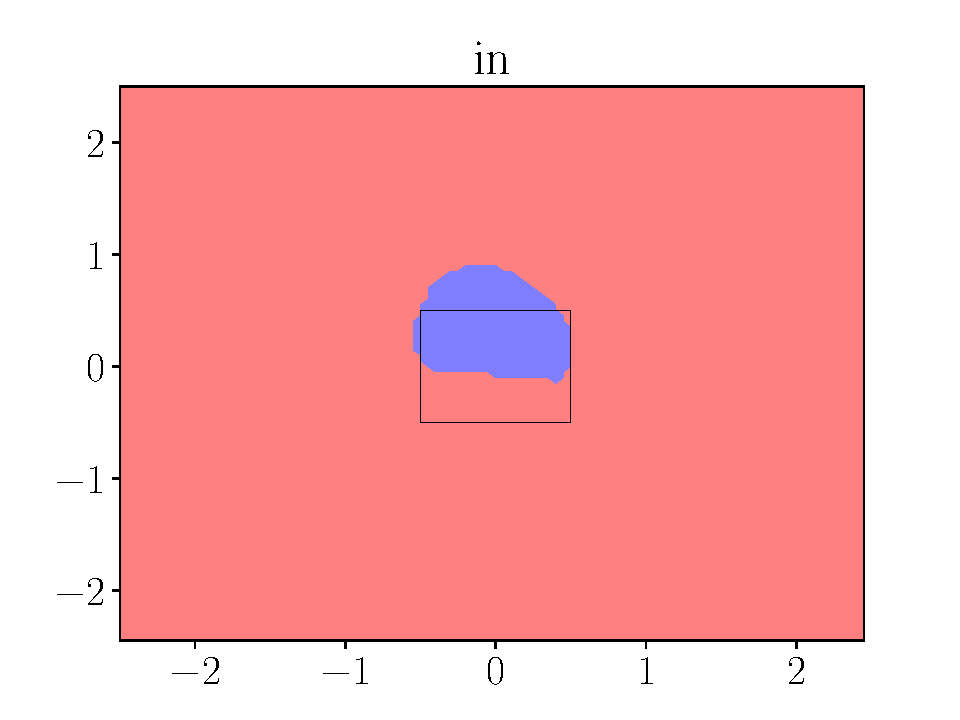
\includegraphics[width=\textwidth]{figures/in_predicate_only.pdf}
        \end{subfigure}
        \begin{subfigure}{0.45\textwidth}
            \centering
            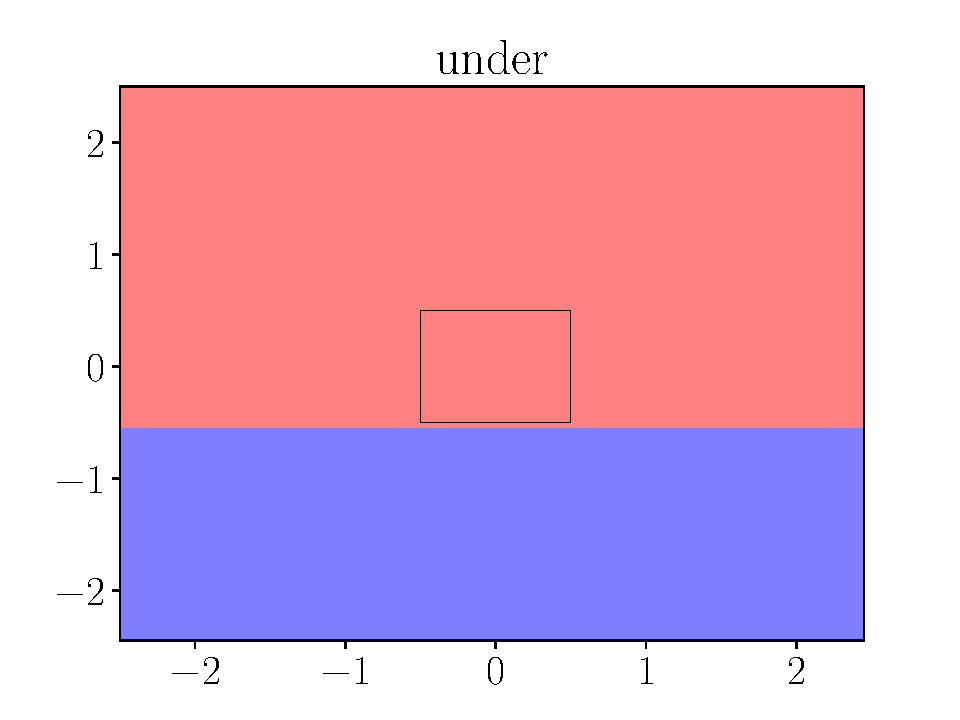
\includegraphics[width=\textwidth]{figures/under_rule.pdf}
        \end{subfigure}
        \begin{subfigure}{0.45\textwidth}
            \centering
            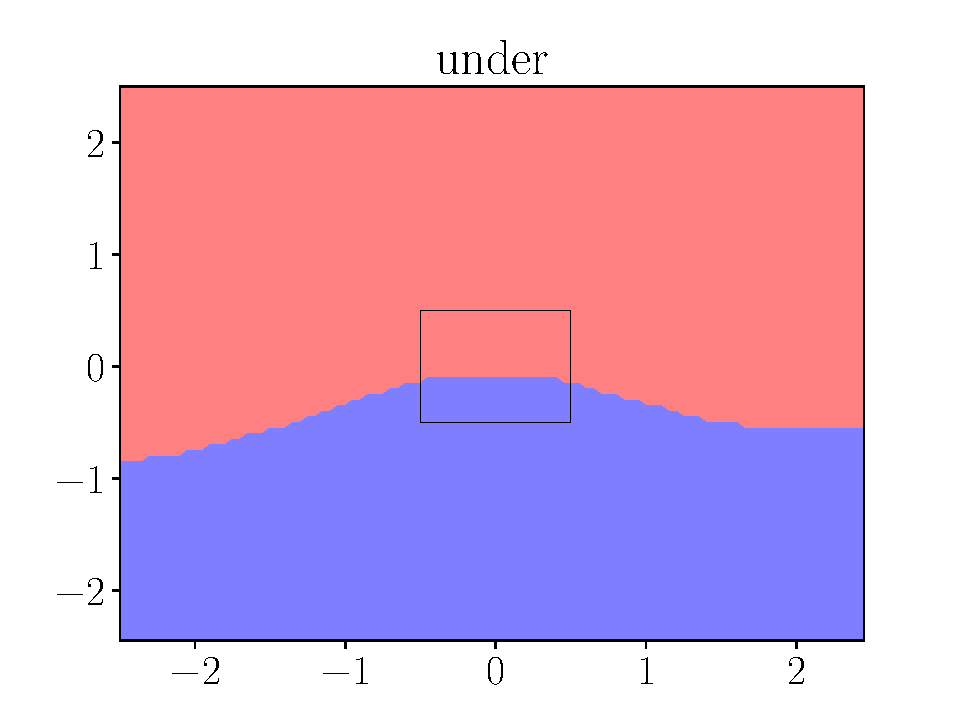
\includegraphics[width=\textwidth]{figures/under_predicate_only.pdf}
        \end{subfigure}
    \caption[Rule-based constraints compared to classifier-based constraints]{Rule-based constraints (on the left) compared to the classifier-based constraints (on the right). The classifier used in these examples was trained using only predicates and the $x$, $y$ coordinates.}
    \label{fig:boundaries:3}
\end{figure}

\begin{figure}[ht]
    \centering
        \begin{subfigure}{0.45\textwidth}
            \centering
            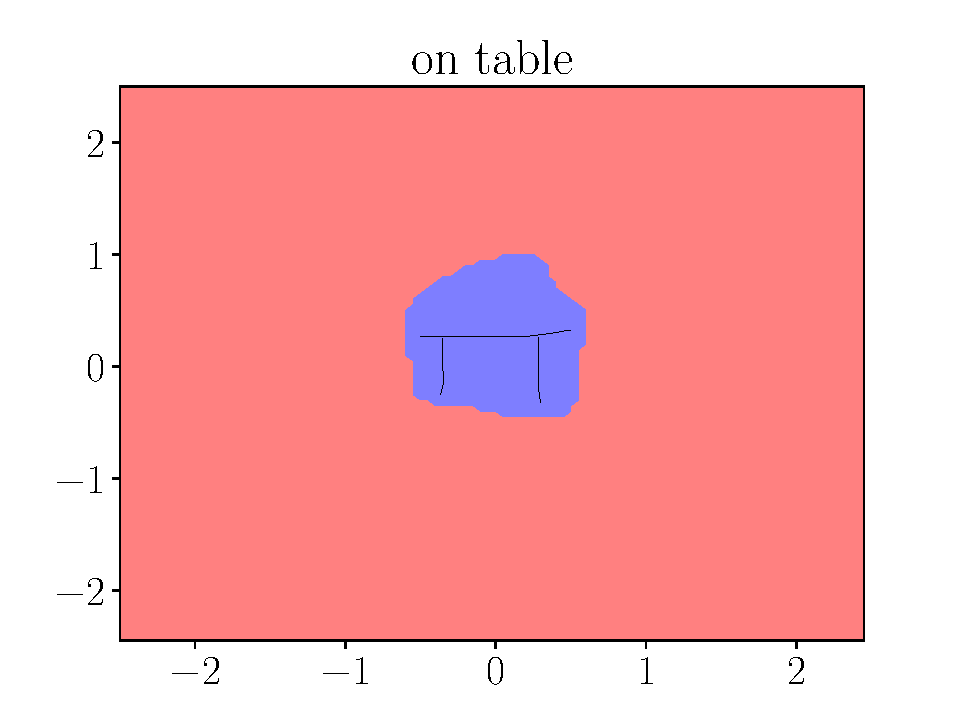
\includegraphics[width=\textwidth]{figures/on_table}
        \end{subfigure}
        \begin{subfigure}{0.45\textwidth}
            \centering
            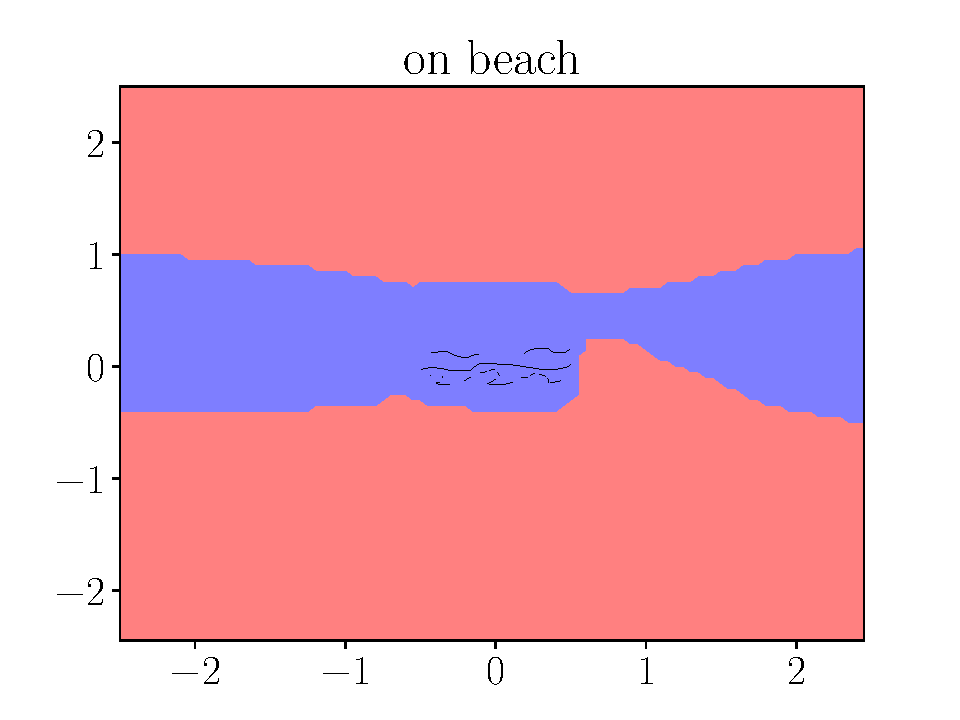
\includegraphics[width=\textwidth]{figures/on_beach}
        \end{subfigure}
    \caption[Different decision boundaries for the same predicate]{Different decision boundaries capture semantic difference of the same predicate in different contexts.}
    \label{fig:boundaries:2}
\end{figure}

\begin{figure}[ht]
    \centering
        \begin{subfigure}{0.45\textwidth}
            \centering
            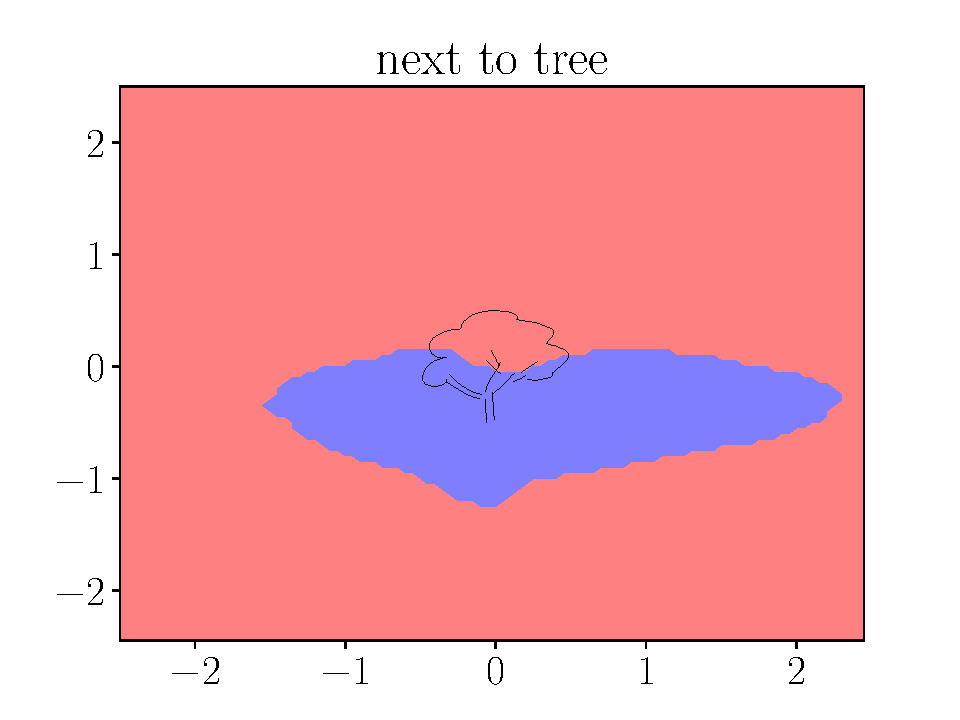
\includegraphics[width=\textwidth]{figures/next_to_tree.pdf}
        \end{subfigure}
        \begin{subfigure}{0.45\textwidth}
            \centering
            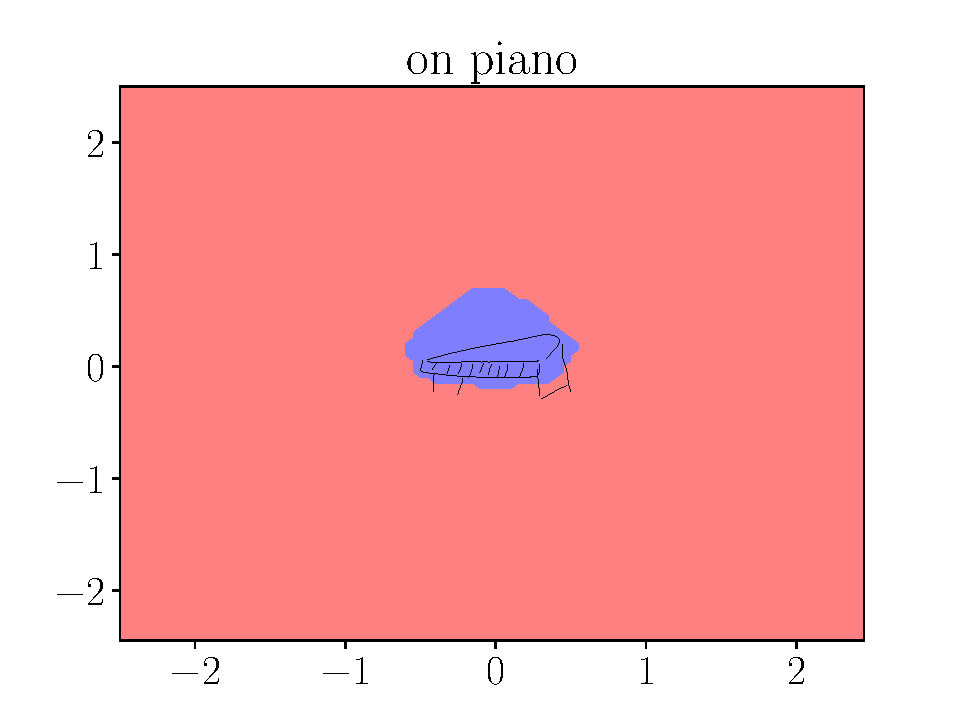
\includegraphics[width=\textwidth]{figures/on_piano.pdf}
        \end{subfigure}
        \begin{subfigure}{0.45\textwidth}
            \centering
            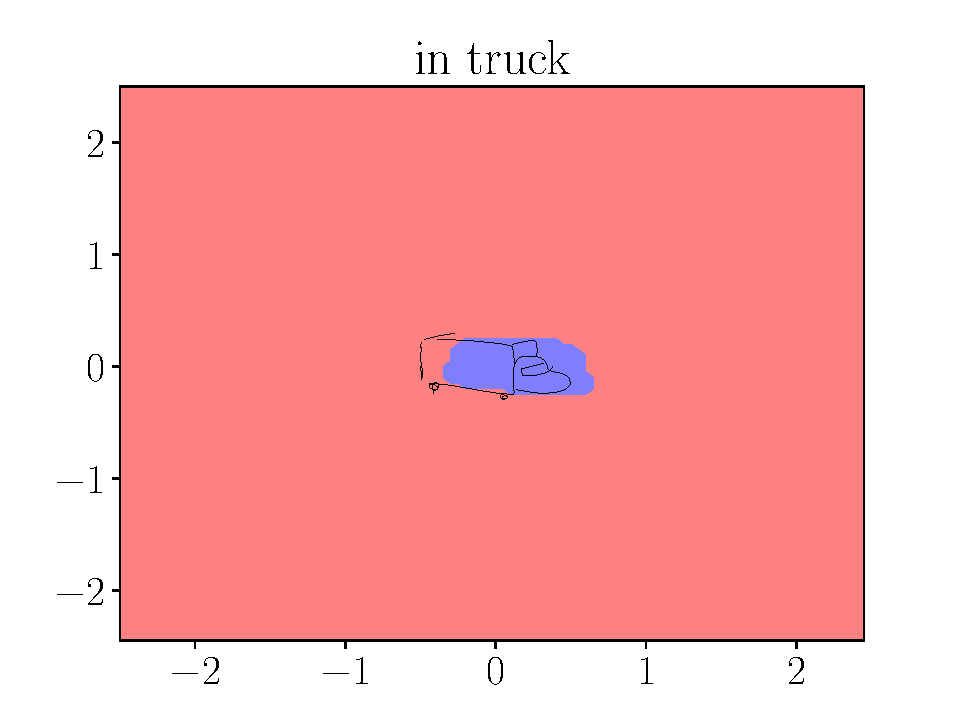
\includegraphics[width=\textwidth]{figures/in_truck.pdf}
        \end{subfigure}
        \begin{subfigure}{0.45\textwidth}
            \centering
            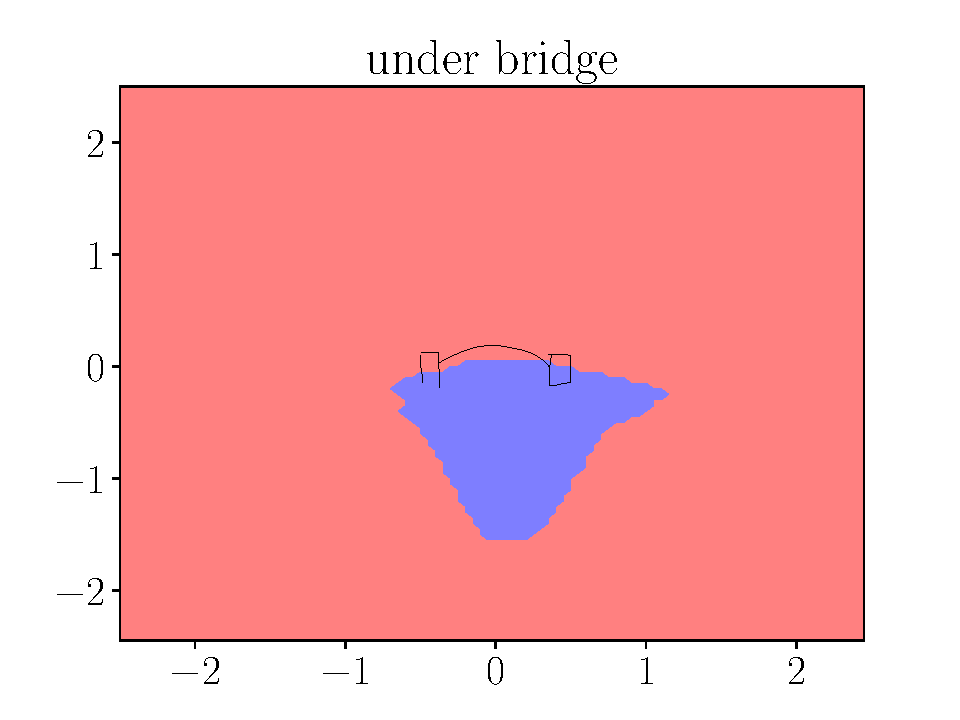
\includegraphics[width=\textwidth]{figures/under_bridge.pdf}
        \end{subfigure}
    \caption[More examples of the classifier-based constraints]{More examples of the classifier-based constraints.}
    \label{fig:boundaries:5}
\end{figure}

\begin{figure}[ht]
    \centering
        \begin{subfigure}{0.45\textwidth}
            \centering
            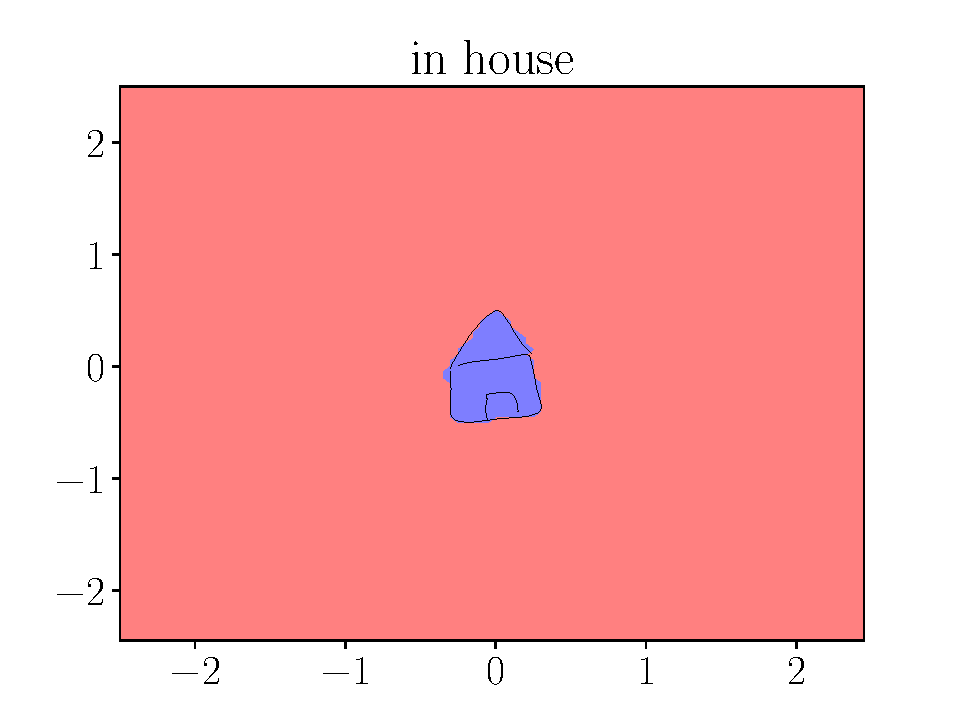
\includegraphics[width=\textwidth]{figures/in_house_rule.pdf}
        \end{subfigure}
        \begin{subfigure}{0.45\textwidth}
            \centering
            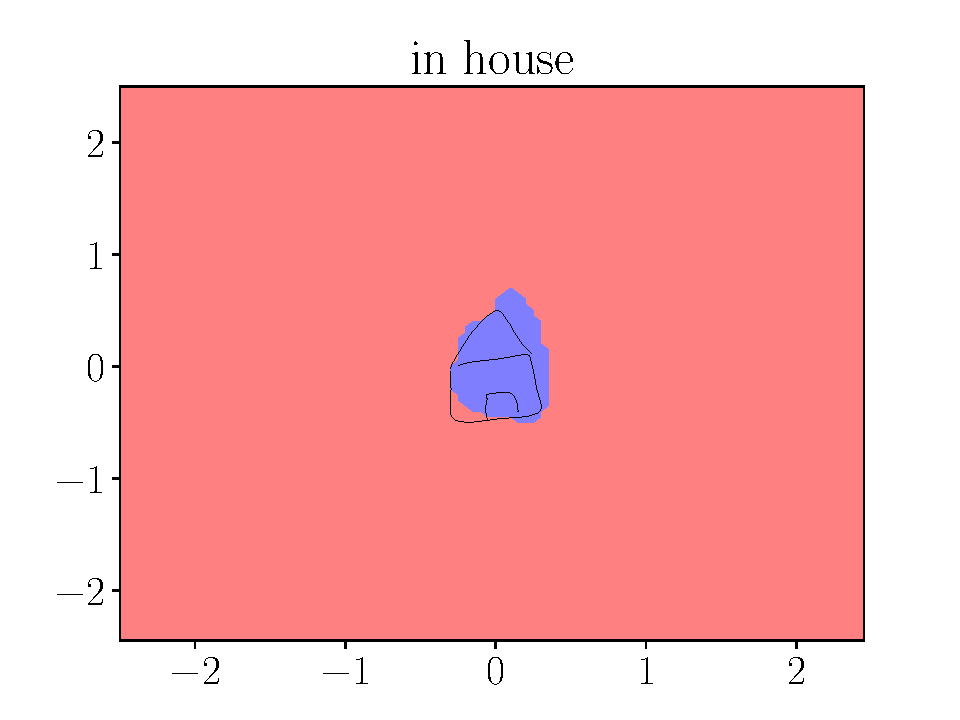
\includegraphics[width=\textwidth]{figures/in_house_classifier.pdf}
        \end{subfigure}
    \caption[\emph{Inside} constraint comparison]{The rule-based \emph{inside} constraint (on the left) can be more precise than the classifier-based one (on the right).}
    \label{fig:boundaries:4}
\end{figure}

